This chapter explains how and why water moves in waves, once the waves have been generated. 
A more logical sequence might have been to study the generation process of the waves first, but it is much more complex 
and can only be understood once one knows how the waves move. The properties exposed in this chapter
are thus common to all surface gravity waves, including tsunamis and wind-generated waves. 

In order to make things simple, we consider a flat, non-deformable bottom 
located at $z=-h$, and periodic waves in both space and time. This may sound very restrictive, but waves at 
sea generally behave as if the bottom were locally flat, and the periodicity allows us to study elementary waves 
that are later superimposed thanks to the quasi-linear wave motion, with some possible non-linear corrections to better fit
the equations of motion. We will thus start with the linear wave theory of unidirectional and monochromatic 
waves that was first developed by  \cite{Airy1841}, and which is a good approximation for waves of small height in not-too-shallow water. 
These are the typical conditions found in swells for depths larger than 50~m or so. Swells are the waves generated by winds in remote storms. 
It is also instructive for the oceanographer to play the game of differences, and find the common traits and main differences 
between these swells, and the tidal waves in shallow water that take the form of  Kelvin waves. In fact, most 
of the wave properties derived here also apply to Kelvin waves. The main difference is the geostrophic balance along the crest of Kelvin waves 
that does not exist for shorter gravity waves for which the Coriolis force can be neglected for most properties. 


We will try here not to get carried away by mathematics, which are necessary to arrive at quantitative predictions.
Instead we will use the equations only as tools to help us reveal the wave motion in terms of forces, pressure and flow, which should 
help us navigate the many simplifying assumptions ot understand the role term. 

\section{Waves: a question of gravity, pressure, mass and vorticity}
Before jumping into equations, we should make a few mechanical remarks. 
There is a motion in and above waves because the crests and troughs of the sea surface, located at $z=\zeta(x,y,t)$, 
correspond to different weights of water, which 
creates a pressure difference. We can already note that these pressure variations 
are of the order of $\rho_w g \zeta$, with $\rho_w$ the water density and $g$ the vertical apparent\footnote{Apparent means that 
this is not just Newton's general gravitation but it also includes the centrifuge acceleration due to the Earth rotation, giving 
$g \simeq 9.81$m s$^{-2}$.} acceleration of gravity. With a 1~m difference in height from crest to trough, 
we get a pressure difference of 10 kPa. What is important for the motion is the pressure \emph{gradient}. With a wavelength 
of 200~m, this gives a crest-to-trough pressure gradient of the order of 100 Pa/m at the same level $z$, 
which drives a horizontal acceleration of 0.1~m/s$^2$. 

The water set in motion flows in an orderly way, following several principles. 
First, the mass of water is conserved, and for the slow velocities considered in this chapter, the flow is 
incompressible, hence non-divergent. We will also consider that the bottom does not deform under the waves. 
As a result, the horizontal convergence between a crest and the next trough must give 
rise to a vertical divergence. Besides, because the waves are generated by pressure forces, and propagated by pressure forces, 
the motion is, in a first approximation, irrotational. The vertical and horizontal velocities are thus strongly constrained by 
these two properties: \textbf{incompressibility} and \textbf{zero vorticity}.

In summary, the free surface position $\zeta$ and gravity determine the near-surface pressure $p$, which gives the horizontal velocity $u$. 
The vertical velocity $w$ is determined from the horizontal velocity using the 
zero divergence and vorticity conditions, and $w$ also modifies the pressure field. We thus can express 
the problem of wave mechanics as a set of four equations for the four unknowns that are $\zeta$, $p$, $u$ and $w$. 
%%%%%%%%%%%%%%%%%%%%%%%%%%%%%%%%%%%%%%%%%%%%%%%%%%%%%%%%%%%%%%%%%%%%%%%%%%%%%
\begin{figure}
\centerline{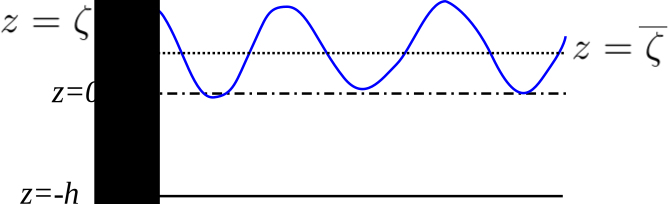
\includegraphics[width=0.5\textwidth]{FIGS_CH_AIRY/vertical_coord_def.pdf}}
%\vspace{3.64in}
  \caption{Definition of vertical levels: $\zeta$ is the sea level, $-h$ is the bottom, both defined relative to an arbitrary vertical datum $z=0$. As a result the
mean water depth is $D=h+\overline{\zeta}$.}
\label{fig:Dandh}
\end{figure}
%%%%%%%%%%%%%%%%%%%%%%%%%%%%%%%%%%%%%%%%%%%%%%%%%%%%%%%%%%%%%%%%%%%%%%%%%%%%%

\section{Wave mathematics}
We shall see that two important quantities, the wavelength $L$ and period $T$ are closely related 
for waves of small amplitude $a$. Here we define "small" to  mean that both the sea surface slope $ka$ and non-dimensional depth $a/D$ are small, 
where $k=2\upi/L$ is the wavenumber, and $D=h+\zb$, is the mean water depth. We remind the reader that $z=-h$
is the vertical position of the bottom, and $\zb$ is the mean sea surface elevation, both relative to an arbitrary datum 
$z=0$.

These small parameters $ka$ and $a/D$ will appear repeatedly in this book. Their ratio gives a third parameter, which is independent 
of the wave amplitude, and that will be very important for the wave kinematics, this is the 
\textbf{non-dimensional depth} $kD$.

We will now go into the details of the linear wave theory, first 
laid out by Airy in the 19th century. It has the great advantages of being  \textbf{linear}, hence any combination of the 
linear solution is also a solution of the equations of motion. More importantly, this linear model explains many of the waves properties, 
and is very accurate for swells in not-too-shallow water, and is not too far off for most wave properties, even for waves 
breaking in the surf zone.  

Let us make two final remarks before we get into the equations. 
First, the linear waves exist only on paper, as all monochromatic waves are unstable, with a development of this instability 
that is faster for higher waves. This aspect is discussed in more details in chapters \ref{ch_sourceterms} and Part 3. 
Monochromatic waves are an acceptable solution for short evolution times, at least a few periods, possibly much more. Second, 
the choice of the Eulerian framework for the equations of motion
is not a very good choice for the accuracy, as the linear Lagrangian theory 
is much more accurate than the Eulerian theory of Airy, because of the very simple balance between the pressure gradient and the 
fluid parcel acceleration.  
\cite{vonGerstner1809} did find an exact theory that exactly satisfies the condition $p=p_a$ at the free surface, 
but it has an non-zero vorticity, which must be compensated by a sheared current. 
The use of Lagrangian equations is unfortunately 
more complex, and this is the main reason why we do not use it here. It is interesting to note, that 
mass conservation is linear in an Eulerian framework, 
while momentum conservation is non-linear, but the opposite is true for a Lagrangian framework. 

\section{Eulerian equations for wave motion}
Our starting point is the conservation of mass and momentum applied to 
the ocean, with the former reduced to a zero divergence as we consider a constant density, which is 
true for the ocean within a few parts per thousand, and incompressible flow. 
The horizontal position is defined by the two-component vector 
${\mathbf x}=\left(x,y\right)$ and the vertical is $z$. The corresponding velocities are 
${\mathbf u}=\left(u,v\right)$ and $w$. Considering sea water as a perfect fluid, 
we apply the Navier-Stokes equations, 
\begin{equation}
    \frac{\partial {\mathbf u}}{\partial t}+{\mathbf u}\bcdot\bnabla{\mathbf u}
    + w \frac{\partial {\mathbf u}}{\partial z}
    =-\frac{1}{\rho_w} \bnabla p +
    \nu \left(\nabla^2 {\mathbf u}+\frac{\partial^2 u}{\partial z^2}\right),
    \label{NSxy}
\end{equation}
\begin{equation}
    \frac{\partial w}{\partial t}+{\mathbf u}\bcdot\bnabla w
    + w \frac{\partial w}{\partial z}
    =-g - \frac{1}{\rho_w} \frac{\partial p}{\partial z} +
    \nu \left(\nabla^2 w+\frac{\partial^2 w}{\partial z^2}\right),
    \label{NSz}
\end{equation}
\begin{equation}
\bnabla\bcdot{\mathbf u} + \frac{\partial w}{\partial z}=0,
\end{equation}
where $\bnabla$ is the horizontal gradient operator. We thus have \textbf{four scalar equations} since \ref{NSxy} has two horizontal components
for the \textbf{four unknowns} that are $u$, $v$,
 $w$ and $p$. Our problem will be well posed as soon as we define the boundary conditions, from the continuity of 
velocity and or stresses (pressure and shear stresses) and initial conditions. At the bottom, we only impose a free slip
 \begin{equation}
w=-{\mathbf u} \bcdot \bnabla h \quad \mbox{at} \quad
z=-h\left({\mathbf x}\right)
\end{equation}
which simplifies to $w=0$ because we chose $h$ to be constant

At the surface, we make the further hypothesis that for any horizontal position $\mathbf{x}$ there is only one value $z=\zeta$ 
of the free surface position (this excludes an overturning of the surface, as found in plunging breakers). 
The free surface is a material surface, which means that water parcels on the surface must stay on the surface. 
This can be expressed by the condition 
\begin{equation}
    \frac{\rm d}{dt}\left(z-\zeta\right)=
    w - {\mathbf u} \bcdot \bnabla \zeta -\frac{\partial \zeta }{\partial t}= 0
    \quad \mbox{at\ }\quad z=\zeta.\label{eq:skbc}
\end{equation}
An interpretation of this surface kinematic boundary condition 
is that the vertical motion 
${\partial \zeta }/{\partial t}$ is the combination of the vertical velocity 
$w$ and the horizontal advection of the water parcels sliding along the surface ${\mathbf u} \bcdot \bnabla \zeta$.

To that kinematic boundary condition we add the dynamic boundary condition that express the continuity of 
stresses at the air-sea interface. Neglecting the wind stress and surface tension, these reduce to a continuity of 
the pressure. In this chapter we will assume that the atmospheric pressure is takes the constant value  $p_a$,
\begin{equation}
    p=p_a\quad \mbox{at\ }\quad z=\zeta.
\end{equation}

We now assume irrotational motion, so that the velocity field 
is given by the gradient of a velocity potential 
$\phi$. Namely, $ {\mathbf u} = \bnabla \phi$ and $w={\partial
\phi}/{\partial z}$. In this and all our notations, the classical operators  (gradient
$\bnabla$, Laplacian $\Delta$ ...) are restricted to the horizontal 
plane, in order to simplify notations. This assumption of irrotational wave motion
is generally consistent with observations of real waves. Still, the vorticity can be 
very strong locally, for example in in the bottom and surface boundary layers
or just after a wave has broken. Also, in the presence of sheared currents, the wave motion always has 
some vorticity, and a weak vorticity also arises from the Earth rotation. 
%Il faut noter que cette condition n'est
%n\E9cessaire qu'\E0 un instant donn\E9: un mouvement initialement
%irrotationnel reste irrotationnel. 
We finally start off by neglecting the viscous terms in the Navier-Stokes equations. This is justified by the 
fact that any significant 
wave-induced motion has scales of velocity $U$ and length $L$ that are large enough to 
make the Reynolds number $UL/\nu$ of the order of  10$^4$ or more.

All the assumptions made above remove some real features in the wave motion. 
Real waves always have some vorticity, which is also linked to the viscosity 
effects in the boundary layers. A rigorous treatment of these effects is possible 
and will be discussed in other chapters. We are here looking for the most 
simple solution that will capture most of the important properties of real waves. 


Replacing velocities by gradients of $\phi$ in
(\ref{NSxy})--(\ref{NSz}) one arrives at
\begin{equation}
    \bnabla \left[\frac{\partial \phi}{\partial t}
    +\frac{1}{2}\left(
    \left|\bnabla \phi\right|^2
    +\left(\frac{\partial \phi}{\partial z}\right)^2
    \right)
    +\frac{p}{\rho_w}+gz \right]=0,
\end{equation}
and
\begin{equation}
    \frac{\partial}{\partial z} \left[\frac{\partial \phi}{\partial t}
    +\frac{1}{2}\left(
    \left|\bnabla \phi\right|^2
    +\left(\frac{\partial \phi}{\partial z}\right)^2
    \right)
    +\frac{p}{\rho_w}+gz \right]=0.\label{eq:NStoBer}
\end{equation}
These two equations establish that the term in brackets is not a function of position and can 
only be a function of time $\gamma(t)$. 

The other important equation given by the conservation of mass is linear, 
The mass conservation equation was already linear, 
\begin{equation}
\bnabla \bcdot {\mathbf u} + \frac{\partial w}{\partial z} =0
\end{equation}
and is equivalent to Laplace's equation for $\phi$
\begin{equation}
    \bnabla^2 \phi + \frac{\partial^2 \phi}{\partial z^2}=0,
    \quad \mbox{at\ }\quad -h\leq z \leq \zeta. \label{Laplace}
\end{equation}


\section{Small slope waves over a flat bottom: the Airy solution}
So far, we had only assumed an incompressible flow (assumption A1), zero viscosity (A2), 
irrotational motion (A3), a flat bottom (A4). 

% and a sinusoidal  et que
%le potentiel des vitesses varie spatialement comme une sinuso\EFde
%(H5). 

We shall now linearize the momentum equations (\ref{eq:NStoBer}), assuming that the wave amplitude is small enough to 
neglect the non-linear terms. This is verified in chapter Part 3, provided that 
the wave amplitude $a$ is much less than the wavelength $L$ and $a$ is much less than the mean water depth $D$. 


This gives the linearized Bernoulli equation
\begin{equation}
    \frac{\partial \phi}{\partial t} \simeq 
       -\frac{p}{\rho_w}-g z + \gamma(t).\label{Bernoulli_lin}
\end{equation}
Assuming that waves are propagating \footnote{In the presence of standing waves, $\gamma(t)$ 
is an oscillating function of the order of $g a^2/L$, as derived by \cite{Miche1944d}.  \cite{Longuet-Higgins1950} further showed that this pressure field is actually an acoustic wave when the water compressibility is considered, which explains the generation of seismic and acoustic waves by ocean wind-generated waves.} at a speed $C$, the motion is periodic as a function of $x-C(t)$ and thus $\gamma(t)$ is a true constant, that can be determined from the dynamic boundary condition $p=\overline{p}_a$ at $z=\zeta$,
This gives the pressure as a function of the velocity potential, for $z< \zeta$, 
\begin{equation}
    p=\overline{p}_a -{\rho_w}g(z-\zeta) 
    -\rho_w \frac{\partial \phi}{\partial t}.\label{p_all}
\end{equation}
The Bernoulli equation states that the pressure is the hydrostatic pressure plus some correction 
due to the non-stationary motion. The static pressure term has been removed by the linearization. 

The linearized kinematic boundary condition, which expresses the continuity of velocities, reads
\begin{equation}
    w = \frac{\partial \phi }{\partial z} \simeq \frac{\partial \zeta}{\partial t}
    \quad \mbox{at\ }\quad z=\zeta,  \label{surface_lin}
\end{equation} which corresponds to a flat sea surface approximation. 
We can further approximate that the actual sea level is not too far from the mean sea level $z=\overline{\zeta}$. 


Finally, the bottom kinematic boundary condition becomes, 
\begin{equation}
    w=\frac{\partial \phi }{\partial z}=0 \quad \mbox{sur\ }\quad z=-h.  \label{bottom}
\end{equation}

Taking  $\partial (\ref{Bernoulli_lin} \textrm{~at z=}\zeta)/\partial t $
+$g\times$(\ref{surface_lin}) we eliminate the unknown $\zeta$, and obtain our 
wave equation 
\begin{equation}
  \frac{\partial^2{\phi}}{\partial{t^2}}+g\frac{\partial\phi}{\partial z}=0, \quad \mbox{at}
\quad  z=\overline{\zeta}. \label{surface 1}
\end{equation}

Equations (\ref{bottom})--(\ref{surface 1}) are the bottom and top boundary conditions for Laplace's equation. The 
set of equation  (\ref{Laplace})--(\ref{surface 1}) is
usually called the Euler equation. Its full non-linear form is given in Part 3. 
 
\subsection{Solution: Laplace equation and vertical profiles}
Since we have a linear wave equation, it is natural to solve it 
using the Fourier transform that gives us a full basis of solutions. Without loss of generality, 
we thus look for solutions of the form, 
\begin{equation}
    \phi=\Re \left(\widetilde{\phi}\left(z\right)
     \mathrm{e}^{\mathrm{i}{\mathbf k}\bcdot{\mathbf x} - \sigma t} \right),
    \label{phi1}
\end{equation}
where $\Re(x)$ is the real part of $x$. Replacing in Laplace's equation gives the Helmolz equation 
\begin{equation}
    -k^2 \widetilde{\phi}+\frac{\partial^2 \widetilde{\phi}}{\partial z^2}=0.
    \label{Helmholz}
\end{equation}
Any solution is thus the sum of two exponentials, which can be recombined in the form 
\begin{equation}
    \widetilde{\phi}(z)=A \cosh\left(kz+kh \right)
        + B \sinh\left(kz+kh \right).
\end{equation}
The bottom boundary condition imposes that $B=0$, and we thus only keep the first term,
\begin{equation}
    \widetilde{\phi}\left(z\right)=\Phi_0
    \frac{\cosh\left(kz+kh\right)}{\cosh\left(kD\right)}.
    \label{cosh}
\end{equation}

Considering that the amplitude of the vertical velocity $w=\partial \widetilde{\phi} / \partial z$ at the surface, where $z+h=D$,  is the radian frequency $\sigma$ times the elevation amplitude $a$, 
we have 
\begin{equation}
    | \Phi_0 |   k \sinh (kD) / \cosh (kD) = \sigma a.
\end{equation}
Hence, from Laplace's equation alone we get the orbital velocities. Wave motion has a maximum horizontal speed at the crest with a magnitude  $\sigma a / \tanh(kD)$, and in the direction 
of propagation. Because of the Laplace equation, when $kD >> 1$ the motion decays exponentially away from the surface over a typical distance that is $1/k=L/2\pi$.

%The only fact that the velocity potential is a solution to Laplace equation gives important analogies with many other waves but also other physical phenomena: electromagnetic waves are also surface waves with "skin effects" when considering high enough frequencies. 


\subsection{Solution: Momementum balance and dispersion relation}
Replacing $\phi$ by eq. (\ref{phi1}) using (\ref{cosh}) in the wave equation (\ref{surface 1}) gives  
\begin{equation}
    - \sigma^2 \Phi_0 +gk\tanh\left(kD\right)\Phi_0=0.
     \label{onde 1}
\end{equation}
This equation expresses the balance of forces between the horizontal pressure gradient which, just below the surface is 
is hydrostatic, with an amplitude  $\rho_w g a k$, and the horizontal acceleration, which has an amplitude  $\sigma^2 a / \tanh(kD)$. 
This is the dispersion relation for linear waves over a flat bottom, first given by \cite{Laplace1776}, 
\begin{equation}
    \sigma^2=g k \tanh\left(kD\right).
     \label{dispersion}
\end{equation}
As a result, where $D$ is reduced but $\sigma$ is constant, waves have a lower phase speed $C=\sigma/k$  for example near the shoreline. 
Contrary to a widespread misconception, this reduction of the phase speed has nothing to do with bottom friction.
in fact the wave orbital velocity increases, and in the Airy theory there is no dissipation of energy.




\subsection{Solution: polarization relations}
Having solved for the velocity potential, we can now link it back to the surface elevation using eq. (\ref{surface_lin}). 
Defining the phase of the free surface elevation, 
\begin{equation}
   \Theta={\mathbf
k}\bcdot{\mathbf x}-\sigma t+ \Theta_0, \label{eq:phase}
\end{equation}
 with $\Theta_0$ a constant between 0
et $2\pi$, eq. (\ref{surface_lin}) links the surface elevation amplitude $a$ and the amplitude $\Phi_{0}$ of the velocity potential at the surface 
\begin{equation}
    a={\mathrm i}\frac{\sigma}{g}\Phi_{0},\label{afromPhi0}
\end{equation}
the elevation, velocities and pressure of the \cite{Airy1841}\footnote{Although 
Laplace, Cauchy and Poisson gave all elements of this theory many years 
before Airy, the latter was the first to address the problem of a single propagating monochromatic 
wave train. Poisson solved several problems of greater complexity, including stationary waves 
and circular waves \citep{Craik2004}.} We thus have  the  following 
polarization relations that link the amplitudes and phase of all oscillating variables 
\begin{equation}
    \zeta-\overline{\zeta}=a \cos \Theta,\label{polzeta}
\end{equation}
and the velocity potential 
\begin{equation}
    \phi=  \frac{a}{k}\sigma
    \frac{\cosh\left(kz+kh\right)}{\sinh\left(kD\right)}
    \sin \Theta.
      \label{potentielcos}
\end{equation}
gives the velocity field
\begin{equation}
    \ub= a \frac{{\mathbf k}}{k}\sigma
    \frac{\cosh\left(kz+kh\right)}{\sinh\left(kD\right)}
    \cos \Theta,
      \label{vitesse}
\end{equation}
\begin{equation}
    w=a \sigma
    \frac{\sinh\left(kz+kh\right)}{\sinh\left(kD\right)}
    \sin \Theta. \label{eq:w}
\end{equation}
The pressure field is obtained from the linearized Bernoulli equation with the constant 
given by the dynamic surface boundary condition, as in eq. (\ref{p_all}), 
\begin{equation}
    p=\overline{p}^H+\rho_w g a
    \frac{\cosh\left(kz+kh\right)}{\cosh\left(kD\right)}
    \cos \Theta,
      \label{pression}
\end{equation}
where the hydrostatic pressure is $\overline{p}^H=-\rho_w g
(z-\zb)+\overline{p}_a$ with ${p}_a$ the atmospheric pressure. 
We also have




%et la fonction de courant
%\begin{equation}
%    \psi=  \frac{a}{k}\sigma
%    \frac{\sinh\left(kz+kH\right)}{\sinh\left(kD\right)}
%    \cos \left({\mathbf k}\bcdot{\mathbf x}-\sigma t + \Theta \right),
%      \label{vitesse}
%\end{equation}


We obtain the displacements of water particles by integrating the velocity field in 
time. To a first order of approximation (at first order in $\varepsilon=ka$),
we have the horizontal displacement
\begin{equation}
     \widetilde{\xi}_h = - a \frac{{\mathbf k}}{k}
    \frac{\cosh\left(kz+kh\right)}{\sinh\left(kD\right)}
    \sin \Theta,
      \label{xi1}
\end{equation} and the vertical displacement
\begin{equation}
    \widetilde{\xi}_3 =a
    \frac{\sinh\left(kz+kh\right)}{\sinh\left(kD\right)}
    \cos \Theta \label{xi3}.
\end{equation}
Because of the wave propagation, the water parcels spend more time under the crest, where the horizontal 
velocity is larger, than under the trough, where the velocity is weaker. As a result there is a net, order $(ka)^2$ drift in the direction 
of propagation, even for linear waves. This is a Stokes drift - it is also called the wave (pseudo)-momentum. Like the energy and the wave action, the Stokes 
drift is an intrinsic quadratic property 
of the wave field. This aspect is discussed in more details in chapter \ref{ch_momentum}. 

Eq. (\ref{dispersion})--(\ref{potentielcos}) are all approximate solutions corresponding to the Airy waves. \cite{Stokes1849} extended this Airy solution 
to take into account the non-linear terms of the full equation (see Part 3), which improves the agreement with observations.
In the deep ocean, all measurements confirm that waves are very nearly irrotational and well described
by the theories of Airy and Stokes
\citep[see for example ][]{Thornton&Kraphol1974,Herbers&al.1992}. The general solution can be expressed as a 
series in powers of 
$\varepsilon_1=ka$, which was shown to converge by \cite{Levi-Civita1925}. Many methods have been developed to 
obtain various numerical approximations of the exact solution.

\subsection{Physical interpretation}
The wave motion is maintained by the restoring force of gravity, which acts in quadrature to the velocity field, 
and thus always overshoots the equilibrium and creates crests where there were troughs. 
The acceleration induced by the pressure field feeds back into the pressure, and the motion \emph{is not} hydrostatic. 
Near the surface, the pressure is nearly hydrostatic (figure \ref{fig:puv1}). If the depth is large enough, 
at some level the vertical acceleration eventually cancels the pressure oscillations so that there is no 
significant motion at a depth much larger than the wavelength. This is typical of a surface wave, the motion decays exponentially 
from the surface, it is 'evanescent' or 'inhomogeneous'. 
%%%%%%%%%%%%%%%%%%%%%%%%%%%%%%%%%%%%%%%%%%%%%%%%%%%%%%%%%%%%%%%%%%%%%%%%%%%%%
\begin{figure}
\centerline{\includegraphics[width=0.6\textwidth]{FIGS_CH_AIRY/2sec_3mdepth_ppuv_1.pdf}}
%\vspace{3.64in}
  \caption{Pressure and velocity fields for a monochromatic wave of 
period $T=2$~s in a mean water depth of  $D=3$~m.}
\label{fig:puv1}
\end{figure}
%%%%%%%%%%%%%%%%%%%%%%%%%%%%%%%%%%%%%%%%%%%%%%%%%%%%%%%%%%%%%%%%%%%%%%%%%%%%%

The flow is better understood by looking at the pressure $p$ 
corrected for a hydrostatic pressure $p^H=p_a-\rho_w g (z-\overline{\zeta})$. This reveals a striking property, 
which is only true for $kD \gg 1$, the isobars of $p-p^H$ are also the streamlines. The streamfunction 
$\psi$ is such that $u=\partial \psi/\partial z$, which gives
\begin{equation}
    \psi=  \frac{a}{k}\sigma
    \frac{\sinh\left(kz+kD\right)}{\sinh\left(kD\right)}
    \cos \Theta,
      \label{potentiel}
\end{equation}
which is, for $kD\rightarrow \infty$ the pressure times $\rho_w g k$. 
This flow is in cyclostrophic equilibrium: the pressure gradient balances the 
centrifugal force of a water parcel turning around its circular orbit. 
%%%%%%%%%%%%%%%%%%%%%%%%%%%%%%%%%%%%%%%%%%%%%%%%%%%%%%%%%%%%%%%%%%%%%%%%%%%%%
\begin{figure}
\centerline{\includegraphics[width=0.9\textwidth]{FIGS_CH_AIRY/2sec_3mdepth_puv_drift.pdf}}
%\vspace{3.64in}
  \caption{Left, in colors: pressure anomaly $p-p^H$ and velocities at different phases 
of the propagation of 2~s period wave in 3~m water depth, going from left to right. 
Right: trajectories of water particles.}
\label{fig:puvdrift}
\end{figure}
%%%%%%%%%%%%%%%%%%%%%%%%%%%%%%%%%%%%%%%%%%%%%%%%%%%%%%%%%%%%%%%%%%%%%%%%%%%%%



%%%%%%%%%%%%%%%%%%%%%%%%%%%%%%%%%%%%%%%%%%%%%%%%%%%%%%%%%%%%%%%%%%%%%%%%%%%%%
\begin{figure}
\centerline{\includegraphics[width=0.7\textwidth]{FIGS_CH_AIRY/10sec_3mdepth_puv_drift.pdf}}
%\vspace{3.64in}
  \caption{Velocity field in water for a wave train of period 10~s, and amplitude 18~cm in 3~m of water. Snapshots are shown for 
(a) $T=0$, (b) 1.25 and (c) 2.5~s. 
The trajectories of water parcels are integrated over two Eulerian periods  (20~s) for (d) linear waves, and (e) nonlinear waves with the 
same period and height, using streamfunction theory (see part 3). For the height chosen here, $H/D=0.12$ and $H/L=0.0067$, so that 
linear theory gives a  fairly good approximation. }
\label{fig:uv2}
\end{figure}
%%%%%%%%%%%%%%%%%%%%%%%%%%%%%%%%%%%%%%%%%%%%%%%%%%%%%%%%%%%%%%%%%%%%%%%%%%%%%



\subsection{Kinematics: influence of the non-dimensional depth $kD$}
The changes in kinematics and dispersion from deep to shallow water are related to the hyperbolic functions $\cosh$, $\sinh$
and $\tanh$, which are plotted in figure \ref{coshsinh}.
%%%%%%%%%%%%%%%%%%%%%%%%%%%%%%%%%%%%%%%%%%%%%%%%%%%%%%%%%%%%%%%%%%%%%%%%%%%%%
\begin{figure}
\centerline{\includegraphics[width=0.5\textwidth]{FIGS_CH_AIRY/coshsinh_en.pdf}}
%\vspace{3.64in}
  \caption{The main hyperbolic functions, used again and again in ocean wave theory.}
\label{coshsinh}
\end{figure}
%%%%%%%%%%%%%%%%%%%%%%%%%%%%%%%%%%%%%%%%%%%%%%%%%%%%%%%%%%%%%%%%%%%%%%%%%%%%%


\subsubsection{Airy waves in deep water}
 A good number to remember is that, at a depth equal to half the
wavelength,  the motion amplitude is reduced by a factor $\exp(\pi) \simeq 25$ compared to the value at the surface.
As a result, waves such that $D > L/2$ which corresponds to $kD > \pi$, are generally considered to be 'deep water waves'.

The dispersion relation becomes, 
\begin{equation}
    \sigma^2 \simeq g k,
     \label{dispersion deep}
\end{equation}
the orbital velocities and pressures become
\begin{equation}
    \ub=a{\mathbf k}\frac{\sigma}{k}
    {\mathrm e}^{kz}    \cos \Theta
\end{equation}
\begin{equation}
    w=a \sigma
    {\mathrm e}^{kz}    \sin \Theta.
\end{equation}
\begin{equation}
    p=\overline{p}^H+ \rho_w g a
    {\mathrm e}^{kz}    \cos \Theta.
\end{equation}
and displacements (\ref{xi1})-(\ref{xi3}) are now
\begin{equation}
    \widetilde{\xi}_h=-a \frac{\mathbf k}{k}
    {\mathrm e}^{kz}  \sin \Theta,
\end{equation}
\begin{equation}
    \widetilde{\xi}_3= a {\mathrm e}^{kz}  \cos \Theta,
\end{equation}
which is the parametric equation of a circle of radius $a {\mathrm e}^{kz}$.
In first approximation, the water parcels follow circular orbits with diameters that vanish with deph. 
 
\subsubsection{Airy waves in intermediate water depth}
For smaller water depths, the orbital velocity is significant near the bottom 
and the trajectories are now ellipses with horizontal major axis measuring 
$2 a
{\cosh\left(kz+kh\right)}/{\sinh\left(kD\right)}$, and 
a vertical minor axis $2 a
{\sinh\left(kz+kh\right)}/{\sinh\left(kD\right)}$ that shrinks from $2a$ at the surface, 
to zero at the bottom where the motion is back and forth along the 
bottom.

In that range there is no asymptotic expression for the dispersion relation and one may use Table \ref{table_dispersion}. 

%%%%%%%%%%%%%%%%%%%%%%%%%%%%%%%%%%%%%%%%%
\begin{table}
  \centering
  \begin{tabular}{cccccc}
\hline
    $Y=X\tanh(X)$ & $X$     & $Y=X\tanh(X)$ & $X$   & $Y=X\tanh(X)$ & $X$\\
 \hline
       0.05    &     0.2255   &     1.30 & 1.4511 &     2.55  &      2.5795   \\
       0.10    &     0.3216   &     1.35 & 1.4934 &     2.60  &      2.6273   \\
       0.15    &     0.3973   &     1.40 & 1.5360 &     2.65  &      2.6753   \\
       0.20    &     0.4627   &     1.45 & 1.5788 &     2.70  &      2.7234   \\
       0.25    &     0.5218   &     1.50 & 1.6218 &     2.75  &      2.7716   \\
       0.30    &     0.5767   &     1.55 & 1.6651 &     2.80  &      2.8200   \\
       0.35    &     0.6284   &     1.60 & 1.7085 &     2.85  &      2.8684   \\
       0.40    &     0.6778   &     1.65 & 1.7523 &     2.90  &      2.9170   \\
       0.45    &     0.7255   &     1.70 & 1.7962 &     2.95  &      2.9657   \\
       0.50    &     0.7717   &     1.75 & 1.8405 &     3.00  &      3.0145   \\
       0.55    &     0.8168   &     1.80 & 1.8850 &     3.05  &      3.0634   \\
       0.60    &     0.8611   &     1.85 & 1.9297 &     3.10  &      3.1123   \\
       0.65    &     0.9046   &     1.90 & 1.9747 &     3.15  &      3.1613   \\
       0.70    &     0.9476   &     1.95 & 2.0199 &     3.20  &      3.2104   \\
       0.75    &     0.9902   &     2.00 & 2.0653 &     3.25  &      3.2596   \\
       0.80    &     1.0324   &     2.05 & 2.1110 &     3.30  &      3.3088   \\
       0.85    &     1.0744   &     2.10 & 2.1570 &     3.35  &      3.3581   \\
       0.90    &     1.1163   &     2.15 & 2.2031 &     3.40  &      3.4075   \\
       0.95    &     1.1580   &     2.20 & 2.2495 &     3.45  &      3.4569   \\
       1.00    &     1.1997   &     2.25 & 2.2961 &     3.50  &      3.5063   \\
       1.05    &     1.2414   &     2.30 & 2.3428 &   &     \\
       1.10    &     1.2831   &     2.35 & 2.3898 &   &     \\
       1.15    &     1.3249   &     2.40 & 2.4370 &   &     \\
       1.20    &     1.3668   &     2.45 & 2.4843 &   &     \\
       1.25    &     1.4088   &     2.50 & 2.5318 &   &     \\
    \hline                  
\hline
\end{tabular}
  \caption{Table of the inverse function of $X \tanh X$. Defining $Y=\sigma^2 D/g$ it gives $k=X/D$, 
which allows to invert the dispersion relation in the absence of current. 
For $Y< 0.05$ one should use $X=\sqrt{Y}$, and for $Y >3.5$ one should use $X=Y$.}\label{table_dispersion}
\end{table}
%%%%%%%%%%%%%%%%%%%%%%%%%%%%%%%%%%%%


\subsubsection{Airy waves in shallow water}
For very shallow water  (say $kD < 0.1$), the dispersion relation 
becomes
\begin{equation}
    \sigma^2=g D  k^2,
     \label{dispersion shallow}
\end{equation}
and the velocities and pressure are 
\begin{equation}
    \ub=a{\mathbf k}\frac{\sigma}{k \sinh(k D)}
        \cos \Theta
\end{equation}
\begin{equation}
    w=a \sigma
    \frac{\left(kz+kh\right)}{\left(kD\right)}    \sin \Theta.
\end{equation}
\begin{equation}
    p=\overline{p}^H+ \rho_w g a     \cos \Theta = p^H.
\end{equation}
This last expression states that the pressure is hydrostatic, just like in 
tidal waves. Tsunamis also nearly follow this shallow water limit. 

 The orbital displacement (\ref{xi1})-(\ref{xi3})
are now
\begin{equation}
    \widetilde{\xi}_h=-a \frac{\mathbf k}{k \sinh(k D)}
    \sin \Theta,
\end{equation}
\begin{equation}
    \widetilde{\xi}_3= a \frac{\left(kz+kh\right)}{\left(kD\right)}  \cos \Theta,
\end{equation}

\subsection{And in the air?}
So far we have solved for the water motion. The same hypotheses of irrotational 
and incompressible flow will, in the air, produce the same equations and solutions. 
The only difference is that the bottom boundary condition is replaced by 
${\mathbf u}\rightarrow0$ as $z\rightarrow\infty$.
The air motion over waves is thus similar to the water motion in deep water waves. 
The air pressure oscillates, with an amplitude that decays exponentially 
with elevation. 
%%%%%%%%%%%%%%%%%%%%%%%%%%%%%%%%%%%%%%%%%%%%%%%%%%%%%%%%%%%%%%%%%%%%%%%%%%%%%
\begin{figure}
\centerline{\includegraphics[width=\textwidth]{FIGS_CH_AIRY/vitesse_air_eau_en.pdf}}
%\vspace{3.64in}
  \caption{(a) Profile of the horizontal and vertical velocities on both sides 
of the sea surface at a wave crest ($x=0$), and (b) velocity field, with the white line indicating 
the position of the free surface. These velocities correspond to waves of amplitude $a=3$~cm, 
period $T=1.5$~s, in $D=3$~m water depth, which correspond to a wavelength 
$L=3.5$~m, and a non-dimensional water depth $kD=3.4$. }
\label{vitesse_air_eau}
\end{figure}
%%%%%%%%%%%%%%%%%%%%%%%%%%%%%%%%%%%%%%%%%%%%%%%%%%%%%%%%%%%%%%%%%%%%%%%%%%%%%

These results were confirmed by the measurements of \cite{Elliott1972a}, who 
found a vertical decay that is slightly faster than $\mathrm{e}^{-kz}$, due to 
the effect of the mean shear in the wind speed. When this shear is taken into account, the
Laplace equation is replaced by the Orr-Sommerfeld equation, as detailed in Part 3.
Besides, the velocity jump at the air-sea interface, gives rise to a boundary layer 
that is laminar for low wave heights and wind speeds \citep{Dore1978}, but becomes turbulent 
otherwise \citep{Perignon&al.2014}, probably leading to an important dissipation of long waves traveling across oceans that is 
discussed in Part 3.

\subsection{Dispersion}
The velocity at which the wave crests or trough propagate 
is called the phase speed and is given by $C=\sigma/k$ which is also equal to the ratio $L/T$. 
Using the dispersion relation (\ref{dispersion}), we can eliminate $\sigma$
\begin{equation}
    C= \frac{\sigma}{k}=\left[ \frac{g}{k}\tanh \left( kD\right)\right]^{1/2}.
\end{equation}
The phase speed is clearly a function of the wavelength, and thus waves are 
dispersive, meaning that wave packets that contain different components will 
spread over a larger space as they propagate, with the long waves traveling 
faster than the shorter waves. As a result, the waves arriving from a distant storm will 
always have a long period at the beginning and the average period will become shorter over time. 

This dispersion property disappears in shallow water  ($ kD << 1$)
where $C$ goes to $\left( gD\right)^{1/2}$, independently of $k$.
On figure \ref{disperlinLT}, this gives a constant slope, for example for $D=10$~m and $T>5$~s).
%%%%%%%%%%%%%%%%%%%%%%%%%%%%%%%%%%%%%%%%%%%%%%%%%%%%%%%%%%%%%%%%%%%%%%%%%%%%%
\begin{figure}
\centerline{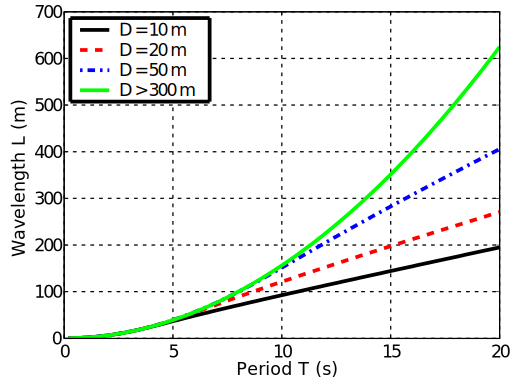
\includegraphics[width=0.8\textwidth]{FIGS_CH_AIRY/disperlinLT_en.pdf}}
%\vspace{3.64in}
  \caption{Wavelength as a function of the wave period and the water depth $D$, for linear waves in the 
absence of currents.}
\label{disperlinLT}
\end{figure}
%%%%%%%%%%%%%%%%%%%%%%%%%%%%%%%%%%%%%%%%%%%%%%%%%%%%%%%%%%%%%%%%%%%%%%%%%%%%%

We also note that, for a fixed period, the phase speed decreases 
with the water depth. This property is also true for a slowly varying water, 
in which case one can consider that the water depth is 'locally constant'. 
This variation of $C$ is the cause of refraction (see chapters \ref{ch_current} and \ref{ch5}). 


\subsection{Energy}
For any water particle, there is an oscillation of the kinetic and potential energies that are exchanged. 
Once integrated over the water depth and averaged over a wave period, that average is represented here by 
the overbar, the potential energy per unit horizontal surface is the vertical integral 
of the potential energy per unit volume $ \rho_w g z$. In practice, we ignore the constant energy between the 
bottom and the mean sea level $\overline{\zeta}$, and we set our reference level such that $\overline{\zeta}=0$,
\begin{eqnarray}
    E_p & = & \overline{ \int_{0}^{\zeta\left(\mathbf{x},t\right)} \rho_w g z {\mathrm d}z }
          = \rho_w g  \overline{ \frac{1}{2} \left(\zeta\right)^2 }   \nonumber\\
    & = & \frac{1}{2} \rho_w g a^2 \overline{ \cos^2\left({\mathbf k} \bcdot {\mathbf x}
    - \sigma t \right) } \nonumber\\
    & = & \frac{1}{4} \rho_w g a^2.
\end{eqnarray}
For the kinetic energy we integrate the kinetic energy per unit volume, $\left( \left|{\mathbf u}\right|^2 + w^2 \right)$ to obtain 
a kinetic energy per unit horizontal surface, 
\begin{eqnarray}
    E_c & = & \overline{  \int_{-h}^{\zeta\left(\mathbf{x},t\right)} \frac{1}{2} \rho_w
\left( \left|{\mathbf u}\right|^2 + w^2 \right) {\mathrm d}z } \nonumber\\
    & \approx & \frac{1}{2} \rho_w \left( \frac{a g k}{\sigma \cosh \left( kD \right)}
    \right)^2 \left[  \overline{ \cos^2 \Theta } \int_{-h}^{\zb} \cosh^2\left(kz+kh\right) {\mathrm d}z 
                   + \overline{ \sin^2 \Theta } \int_{-h}^{\zb} \sinh^2\left(kz+kh\right) {\mathrm d}z     \right] \nonumber\\
    & \approx & \frac{1}{4} \rho_w \left( \frac{a g k}{\sigma \cosh \left( kD \right)}
    \right)^2 \int_{-h}^{\zb} \cosh\left(2kz+2kh\right) {\mathrm d}z \nonumber \\
    & \approx & \frac{1}{4} \rho_w \left( \frac{a g k}{\sigma \cosh \left( kD \right)}
    \right)^2 \frac{\sinh 2kD}{2k}  \nonumber \\
    & \approx & \frac{1}{4} \rho_w g a^2,
\end{eqnarray}
\begin{equation}
    E_t= E_c+E_p= \frac{1}{2} \rho_w g a^2 = \rho_w g  E  ,\label{Etot}
\end{equation}
where $E$ is the variance of the sea surface elevation, here $E=a^2 /2$. 
We have thus found that, to a first order of approximation, the average kinetic and potential energy 
 $E_c$ and $E_p$ are equal. 

Wave propagation is associated to a flux of energy. This flux of energy is transmitted by pressure forces
from one water column to the next. This flux is the work 
of pressure forces given by eq. (\ref{pression}) with a velocity given by eq. (\ref{vitesse}). 
When integrated over the depth and averaged over a wave period, this gives the flux per unit crest length (i.e. per unit horizontal 
distance in the direction perpendicular to the propagation direction), 
\begin{eqnarray}
    W & = & \overline{ \int_{-h} ^{\zeta} p u \mathrm{d}z } \nonumber \\
        & = & \rho_w g a^2 \sigma
        \overline{ \cos^2\left({\mathbf k} \bcdot {\mathbf x} - \sigma t \right)  }
        \int_{-h} ^{\zeta} \frac{\cosh^2 \left(kz+kh \right)}{\sinh kD \cosh kD}
        ~ \mathrm{d}z \nonumber \\
        & = & E_t \frac{2  \sigma}{\sinh (2 kD)}
        \int_{-h}^{\zb} \frac{1}{2}\left[\cosh \left(2kz+2kh\right) +1 \right]
        \mathrm{d}z \nonumber \\
        & = & E_t \frac{2  \sigma}{\sinh (2 kD)}
        \left(\frac{\sinh 2kD}{4k}+\frac{D}{2} \right) \nonumber \\
        & = & C_g E_t \label{W}
\end{eqnarray}
where
\begin{equation}
C_g=\frac{\sigma}{k}
        \left(\frac{1}{2}+\frac{kD}{\sinh 2kD}\right)= C \left(\frac{1}{2}+\frac{kD}{\sinh 2kD}\right). \label{Cg}
\end{equation}
$W$ is a flux of energy per unit distance and $C_g$ the average speed at which the energy density $E_t$ is radiated, 
which defines the group speed. 

The full expression for the energy flux should also include the advective flux  $u \left[\rho_w g z + 0.5\left(u^2 +
w^2\right) \right]$, but that part is negligible in the absence of currents. 
%%%%%%%%%%%%%%%%%%%%%%%%%%%%%%%%%%%%%%%%%%%%%%%%%%%%%%%%%%%%%%%%%%%%%%%%%%%%%
\begin{figure}[htb]
\centerline{\includegraphics[width=0.7\textwidth]{FIGS_CH_AIRY/groups_5_10_en.pdf}}
%\vspace{3.64in}
  \caption{Wave groups produced by the superposition of two monochromatic waves. The top panel corresponds to  $\Delta \sigma/\sigma=0.2$, and the bottom panel
 $\Delta \sigma/\sigma=0.1$. The narrower the spectrum, the larger the number of waves in the group.}
\label{groupes}
\end{figure}
%%%%%%%%%%%%%%%%%%%%%%%%%%%%%%%%%%%%%%%%%%%%%%%%%%%%%%%%%%%%%%%%%%%%%%%%%%%%%

%%%%%%%%%%%%%%%%%%%%%%%%%%%%%%%%%%%%%%%%%%%%%%%%%%%%%%%%%%%%%%%%%%%%%%%%%%%%%
\begin{figure}
\centerline{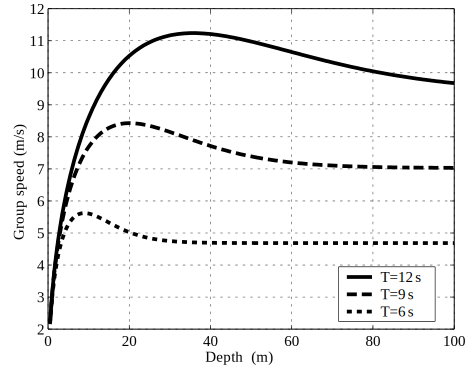
\includegraphics[width=0.55\textwidth]{FIGS_CH_AIRY/cg_en.pdf}}
%\vspace{3.64in}
  \caption{Group speed variation for different periods, as a function of the water depth.}
\label{Cgplot}
\end{figure}
%%%%%%%%%%%%%%%%%%%%%%%%%%%%%%%%%%%%%%%%%%%%%%%%%%%%%%%%%%%%%%%%%%%%%%%%%%%%%

This speed is called 'group speed' because it is indeed the speed at which a group of waves travels, because $C_g=\partial
\sigma/\partial k$. Indeed, the superposition of two monochromatic waves of equal amplitude and similar frequencies gives a surface elevation 
\begin{equation}
    \zeta=a  \cos \left[ \left(k - \Delta k \right) x - \left(\sigma-\Delta \sigma \right) t \right]
        + a  \cos \left[ \left(k + \Delta k \right) x - \left(\sigma+\Delta \sigma \right) t\right]  ,
\end{equation}
which writes
\begin{equation}
    \zeta=2 a \cos \left(\Delta k x -\Delta \sigma t\right)
    \cos \left( k x - \sigma t\right).
\end{equation}
The first factor is the envelope of the group, with a length  $2 \pi /
\Delta k $ and period $2\pi / \Delta \sigma$, that propagates at the speed 
$c'=\Delta \sigma /\Delta k $. This speed is, in the limit  $\Delta k \rightarrow 0$, equal to 
$C_g=\partial \sigma/\partial k$. Two examples are shown in figure 
\ref{groupes}.


We note that for $kD\rightarrow\infty$, equation (\ref{Cg}) gives
$C_g={\sigma}/({2k})=C/2$. Thus, in deep water the groups of waves travel at a speed that is half of the phase speed. 
Things are very different in shallow water ($kD
\ll 1$), where $C_g=C$. In that shallow water limit, waves of all frequencies travel at the same speed (they are not dispersive)
hence the groups also travel at that same speed. This is only true for linear waves. In part 3you may see that  phase and group speeds 
are also a function of the wave amplitude. 


\subsection{Energy and power}
Eq. (\ref{W}) gives the mean energy flux per unit crest length. 
For example, in the case of monochromatic waves with a height of 2~m, a period of 12~s and
a water depth of 15~m, this flux is 
$W\approx 50$~kW~m$^{-1}$. This means that if we take a surface facing the waves, 1 meter along the crest and the full water depth, there is 50~kW of mechanical power that goes through this surface. 
This is 5~MW for 100~m along the crests, which is the peak power of two  150~m high windmills. This number, for rather modest wave heights, 
shows the strong concentration of power in water waves. Unfortunately, this power is difficult to tap to produce electricity, in particular because it is very intermittent in most places.

\subsection{Summary}
We have obtained the main properties of regular linear waves,  summarized in table 
(\ref{table_theory}). Because these Airy waves are solutions of the linearized equations of motion, 
they can be combined to obtain the general solution. Hence the surface elevation, velocities and pressure 
are given by the sum of monochromatic waves, each proportional to their amplitude $a$. We will see in the next chapter that it is also possible to add up the quadratic properties 
that are the energy and Stokes drift, which are  proportional to the surface elevation variance
$E=a^2/2$.
%%%%%%%%%%%%%%%%%%%%%%%%%%%%%%%%%%%%%%%%%%%
\begin{table}
  \centering
  \begin{tabular}{lccc}
\hline
  Water depth: & general case       & $kD \gg 1$  & $kD \ll 1$  \\
\hline
  dispersion relation  &   $\sigma^2=g k \tanh (kD)  $               & $ \sigma^2=g k$ & $\sigma^2=g D k^2 $ \\
  phase speed & $C= {\sigma}/{k}=\left[g  \tanh (kD)/ k\right]^{1/2}$         & $C=\left(g / k\right)^{1/2} ={g}/{\sigma}  $   & $ C = \sqrt{gD}^{1/2}$ \\
  group speed  &  $C_g=C \left(0.5+\frac{kD}{\sinh(2kD)}\right)  $               & $C_g=C/2 $&
  $C_g=C$\\
\hline
  Linear properties  ($z<\zeta$) &    &  & \\
\hline
  horizontal velocity & $\ub =   a \frac{{\mathbf k}}{k}\sigma
    \frac{\cosh\left(kz+kh\right)}{\sinh\left(kD\right)}
    \cos \Theta $         &  $\ub=\frac{a \kb \sigma}{k} \er^{kz}    \cos \Theta$ & $\ub=\frac{a \kb \sigma}{k^2 D}
        \cos \Theta $\\
  vertical velocity & $w =   a \sigma
    \frac{\sinh\left(kz+kh\right)}{\sinh\left(kD\right)}
    \sin \Theta $         &  $w =a \sigma \er^{kz}    \sin \Theta$ & $w=\frac{z+h}{h}{a \sigma} \sin \Theta $\\
\hline
  Quadratic properties &    &  & \\
\hline
 Mean energy per unit surface & $E_t =  \rho_w g E = \rho_w g a^2 /2$  & $E_t =  \rho_w g  a^2 /2$ & $E_t =  \rho_w g  a^2 /2$ \\
 Stokes drift & ${\mathbf U}_s=\sigma \kb E \frac{\cosh(2kz+2kh)}{\sinh^2(kD)}$  & ${\mathbf U}_s=2 \sigma \kb E \er^{2kz} $ & ${\mathbf U}_s=\sigma \kb E /(kD)^2$ \\
\hline
\end{tabular}
  \caption{Main results of Airy wave theory with deep and shallow water limites.  We remind that the phase is  $\Theta={\mathbf
k}\bcdot{\mathbf x}-\sigma t+ \Theta_0$.
}\label{table_theory}
\end{table}
%%%%%%%%%%%%%%%%%%%%%%%%%%%%%%%%%%%%
These properties come from a series of assumptions, listed in table \ref{table_H} and that will be discussed or removed in 
the following chapters that extend Airy theory, giving access to all sorts of corrections and allowing to determine the 
evolution of Airy waves caused by different forcing and dissipation processes. Indeed, we have determined here the 
eigenvectors of the linearized equations of motion: these are free waves that can exist without forcing. In practice, the forcing 
is necessary to generate these waves in the first place, and this forcing is balanced by dissipation when long time scales and large 
spatial scales are considered. That dissipation requires to include vorticity and viscous effects. 
%%%%%%%%%%%%%%%%%%%%%%%%%%%%%%%%%%%%%%%%%%%
\begin{table}
  \centering
  \begin{tabular}{lcc}
\hline
 Assumption          & justification                                  & consequences  \\
\hline
 A1. incompressible &   $u \ll \alpha_w $             & $\bnabla \bcdot \ub + \partial w/\partial z=0$ \\
 A2. rigid bottom   & bottom motion $\ll$ water motion & $w=-\ub \bcdot \bnabla h$ at $z=-h$ \\
 A3. inviscid       & high Reynolds number                    & viscous stresses are zero \\
 A4. irrotational   & motion driven by pressure forces + (A3)   & $\ub=\bnabla \phi$, $w=\partial \phi/\partial z$\\
 A5. flat bottom    & bottom slopes usually $\ll$ 1 & with A2, $w=0$ at $z=-h$ \\
 A6. sine wave      & basis function of the Fourier transform & $\phi(z) \propto
 \cosh(kz+kh)$ \\
 A7. $p_a$ constant on $z=\zeta$ & $\rho_a \ll \rho_w$         &  no wave generation by the wind \\
 A8. no surface tension & $\gamma \ll g/k^2$ for $L \gg 0.1$~m (in clean water) & no capillary waves \\
 A9. $\varepsilon_1=ka \ll 1$ & $\varepsilon_1 <0.44$ for periodic waves & with A10, gives linear equations \\
 A10. $\varepsilon_2=a/D \ll 1$ & because it makes equations simpler & ... but beware for  $kD < 1$! \\
 A11. no mean current & most often $U \ll C$  for dominant waves & simple dispersion  $\sigma^2 = gk \tanh(kD)$ \\
 A12. constant density & $\rho'/\rho_w < 0.03$ for sea water   & no internal waves\\
 A13. no Earth rotation  & $f_3 \ll \sigma $          & \\
 \hline
\end{tabular}
  \caption{Assumptions needed to derive Airy's theory. $ \alpha_w$ is the sound speed in water, of the order of 
1500~m~s$^{-1}$ (in the absence of air bubbles), and $U$ is the mean current velocity. Finally $\rho'$ 
is a scale for density perturbations relative to the mean $\rho_w$, and 
 $\gamma$ is the surface tension, such that $\gamma \rho_w (R_1+R_2)$ is the additional pressure under a surface with radii of 
curvature $R_1$ et $R_2$, counted positive for a surface that is convex on the air-side, e.g. a crest.}\label{table_H}
\end{table}
%%%%%%%%%%%%%%%%%%%%%%%%%%%%%%%%%%%%

\subsection{Extending Airy wave theory}
What happens when we do not make one of the assumptions A1 to A13? In which conditions should we do this? 
\begin{itemize}
  \item A1. Except when considering acoustic and seismic noise generated by ocean waves, as in part 3, we can 
safely ignore compressibility effects. \vspace{0.3cm}
  \item A2. Bottom deformations are relevant when considering acoustic and seismic noise generation. In fact, the bottom 
deformation should be considered for all acoustic wave propagation in the ocean.  \vspace{0.3cm}
  \item A3. In the boundary layers at the sea surface, and more importantly at the sea bottom, 
we will need molecular viscosity and turbulence effects (which can often be represented by an eddy viscosity). 
However, these layers are very thin, with a thickness of the order of 
  $\delta=(\nu/\sigma)^{1/2}$, which is typically less than a millimeter for the kinematic viscosity of water 
$\nu \simeq 4\times 10^{-6}$~m$^2$~s$^{-1}$, and wave periods 
   $T > 1$~s, which is consistent with measurements of the water-side surface boundary layer by \cite{Banner&Peirson1998}. At the bottom, 
turbulence effects are important but the wave boundary layer is only a few centimeters thick.\vspace{0.3cm}
  \item A4. For a viscous flow, the vorticity from the top and bottom boundary layers diffuses in the water column 
and in the air \citep{Longuet-Higgins1953,Weber&Forland1990}. Besides, there is also a weak vorticity caused by the 
Earth rotation, see A13 below. \vspace{0.3cm}
  \item A5. The bottom boundary condition becomes $-\bnabla \phi \bcdot \bnabla h = \partial \phi/\partial z$ (inviscid case), 
and is only satisfied exactly in the presence of at least two wave trains, one incident and one reflected. The incident wave train 
is also modified by diffraction effects.
  For small slopes, diffraction and reflection are generally weak, 
and the wave motion is well approximated by a "WKBJ" approximation: replacing the phase  $\Theta$ by a function  $S(\xb,t)$ 
with $\kb=\bnabla S$ and $\sigma=-\partial S/\partial t$ (see chapter 
  \ref{ch5}). In this context \emph{small} means that refraction or diffraction effects do not produce of significant variation 
of the wave amplitude at the scale of one wavelength. A more accurate approximation of the dispersion relation 
over a sloping bottom was given by 
   \cite{Ehrenmark2005}, in the form 
   $\sigma^2=gk \tanh(kh \beta /\tan \beta)$, where $\beta$ is the angle between the bottom and the horizontal. This correction is 
weak, only 4\% for a slope $\beta=10^\circ$. For steep slopes, reflection becomes important and the separation of the 
variables $\xb$ and $z$ becomes meaningless. The velocity potential can be obtained numerically 
  \citep[e.g.][]{Athanassoulis&Belibassakis1999,Belibassakis&al.2001}.\vspace{0.3cm}
  \item A6. For a flat bottom this is not an assumption: we have the right to decompose the waves into sine waves because these 
are a complete basis. For small bottom slopes, the wave train is only \emph{locally} equivalent to a sine wave. 
For steep slopes, the wave train can suffer strong distortions at the scale of one wavelength \citep[e.g.][]{Magne&al.2007}.\vspace{0.3cm}
  \item A7. An atmospheric pressure oscillation on the scale of the wavelength can produce an amplification or attenuation of the waves, depending 
on its phase relative to the waves. This aspect is discussed in detail in chapters \ref{ch_sourceterms} and Part 3. \vspace{0.3cm}
  \item A8. Due to surface tension, the pressure under the surface is increased by  $-\gamma \left(\partial^2 \zeta/\partial x^2+\partial^2 \zeta/\partial
  y^2\right)$. This added pressure modifies the dispersion relation to give $\sigma^2=\left(gk+\gamma k^3\right) \tanh(kD)$. 
  This modification is negligible for wavelengths larger than a few centimeters. The presence of a layer of ice at the sea surface 
has a similar effect on the waves, with added terms due to bending and inertia, and is significant for periods of 10~s and 
less \citep{Liu&MolloChristensen1988} in the case of an ice layer thickness of one meter or more, and  thicker layers have an influence on longer waves.
  \item A9. Non-linear effects associated to $\varepsilon_1 \neq 0$ are fairly complex and will be 
discussed in chapters \ref{ch_sourceterms} and part 3. 
One particular consequence is that a monochromatic wave train is generally 
unstable \citep{Benjamin&Feir1967}. For waves in one dimension, as produced in the laboratory, 
this can create very high (freak) waves. Another consequence is that different wave trains interact, 
exchanging energy an momentum.\vspace{0.3cm}
 \item A10. Non-linear effects associated to  $\varepsilon_2 \neq 0$ are important for $kD<1$ even if the wave height is small. 
This is particularly true near the shoreline, and the shape of waves can be strongly modified, as discussed in chapters \ref{ch_surf} and 
part 3.\vspace{0.3cm}
 \item A11. Since the laws of physics are unchanged by a change of Galilean reference frame, 
a uniform current $\Ub$ in the absence of bottom friction only introduces a Doppler frequency shift, 
and all results established here remain valid, replacing 
$\Theta$ by $\Theta_D=\Theta+\kb \bcdot
 \Ub$. One can define an absolute frequency, as measured in the reference frame attached to the bottom, 
 \begin{equation}
    \omega=\sigma+\kb \bcdot \Ub =\kb \bcdot \Ub + \left[g k \tanh\left(kD\right)\right]^{1/2}.
     \label{dispersionD}
\end{equation}
For a current   $\Ub(z)$ that varies only in the vertical, and in the limit  $\varepsilon_1 \ll 1$  and $\varepsilon_2 \ll 1$, 
this dispersion relation generalizes to the form,
 \begin{equation}
    \omega\equiv\sigma+\kb \bcdot \Ub_A      \label{dispersionD2}
\end{equation}
with the advection speed given by \cite{Kirby&Chen1989}, 
 \begin{equation}
 \Ub_A   = \kb \bcdot \int_{-h}^{\zb} \Ub(z) \frac{2  k
\cosh\left[2k(z+h)\right]}{\sinh(2kD)} \dr z. \label{dispersionD3}
\end{equation}
Finally, when $\Ub$ also varies horizontally, the phase speed varies horizontally, so that refraction and diffraction effects 
appear, just like they do on a sloping bottom. These questions are addressed  in  chapter \ref{ch_current}.\vspace{0.3cm}
\item A12. When the ocean is stratified, due to a vertical variation of temperature and/or salinity, the Airy waves are the 'external mode' in a family of waves that also include internal waves. 
Because the equations of motion are weakly nonlinear, these different modes are coupled, with an exchange of energy between surface waves and internal waves 
\citep{Thorpe1966}. This aspect is still relatively unexplored  \citep{Osborne&Burch1980,Kudryavtsev1994}. This stratification can also be due to the 
presence of air bubbles near the surface or sediments near the bottom, with important consequences for the bottom boundary layer and wave dissipation. 
\citep[e.g.][]{Winterwerp2007,Styles&Glenn2000}.\vspace{0.3cm}
\item A13. Taking into account the Earth rotation with a vertical Coriolis parameter $f_3$, a very weak transversal velocity component $v$ appears, 
of the order  $f_3 u /\sigma$ and in phase with $w$.  This transversal component is important for the surface drift current
 \citep{Hasselmann1970,Xu&Bowen1994,Ardhuin&al.2004b,Rascle&Ardhuin2009}. In the case of wind-generated waves, 
  $f_3/\sigma$ is typically of the order of 10$^{-4}$, so that the effect on the wave kinematics and dispersion is not measurable. 
There is also a very weak deviation of the propagation direction of the waves \citep{Backus1962}. This is still true for tsunamis 
which have much larger periods than wind-waves, typically a few minutes up to 30 minutes. Airy wave theory thus also applies to tsunamis, as long as non-linear effects are 
weak. On the contrary, for motions with longer periods, such as tides, the Earth rotation must be taken into account. This is why these waves are called inertia-gravity waves. 
\end{itemize}


